\documentclass{standalone}
\usepackage{tikz}

\begin{document}
\begin{minipage}{0.75\textwidth}
\centering
\scalebox{0.7}{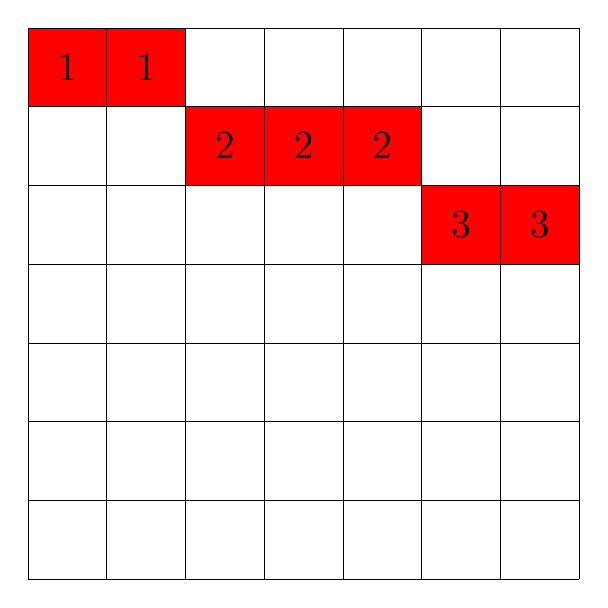
\begin{tikzpicture}
	\foreach \x in {0,1}
	\fill[red] (-1+\x,6) rectangle (0+\x,7);  
	\foreach \x in {0,1,2}
	\fill[red] (1+\x,5) rectangle (2+\x,6);   
	\foreach \x in {0,1}
	\fill[red] (4+\x,4) rectangle (5+\x,5); 

	\node at (-0.5,6.5) {\Large{1}}; 
	\node at (0.5,6.5) {\Large{1}}; 
	
	\node at (1.5,5.5) {\Large{2}}; 
	\node at (2.5,5.5) {\Large{2}}; 
	\node at (3.5,5.5) {\Large{2}}; 
	
	\node at (4.5,4.5) {\Large{3}}; 
	\node at (5.5,4.5) {\Large{3}}; 
	
	\draw[step=1cm,black,very thin] (-1,-0) grid (6,7);
\end{tikzpicture}}
\hspace{1cm}
\scalebox{0.7}{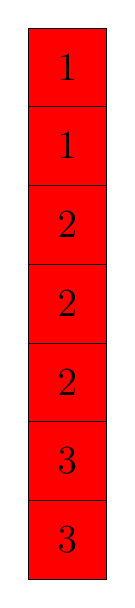
\begin{tikzpicture}
	\foreach \x in {0,1,2,3,4,5,6}
	\fill[red] (8,\x) rectangle (9,\x+1);  
	\draw[step=1cm,black,very thin] (8,-0) grid (9,7);
	\node at (8.5,6.5) {\Large{1}}; 
	\node at (8.5,5.5) {\Large{1}}; 
	\node at (8.5,4.5) {\Large{2}}; 
	\node at (8.5,3.5) {\Large{2}}; 
	\node at (8.5,2.5) {\Large{2}}; 
	\node at (8.5,1.5) {\Large{3}}; 
	\node at (8.5,0.5) {\Large{3}}; 
\end{tikzpicture}}
\end{minipage}
\end{document}
